\documentclass[titlepage, 11px, a4paper]{report}

\usepackage[utf8]{inputenc}

\usepackage[T1]{fontenc}
\usepackage{fontawesome}
\usepackage{eurosym}

\usepackage[french]{babel}

\usepackage{fancyhdr}
\usepackage{graphicx}
\usepackage[left=4.5cm,right=4cm,top=4.5cm, textheight=17cm]{geometry}
\usepackage{wrapfig}

\usepackage{eso-pic}
\usepackage{transparent}

\usepackage{hyperref}
\usepackage{setspace}

\usepackage{titletoc}
\usepackage{titlesec}

\usepackage{stackengine,xcolor}
\usepackage{enumerate}

\titleclass{\part}{top}
\titleformat{\part}[display]
  {\normalfont\huge\bfseries}{\centering\partname\ \thepart}{20pt}{\Huge\centering}
\titlespacing*{\part}{0pt}{50pt}{40pt}
\titleclass{\chapter}{straight}
\titleformat{\chapter}[display]
  {\normalfont\huge\bfseries}{\chaptertitlename\ \thechapter}{20pt}{\Huge}
\titlespacing*{\chapter} {0pt}{50pt}{40pt}

%\usepackage{titlesec}
%\titleformat{\part}[display]
  %{\normalfont\bfseries}{}{0pt}{\Large\bfseries}

\newcommand\BackgroundPic{%
	\put(0,-50){%
		\parbox[b][\paperheight]{\paperwidth}{%
			%\vfill
			\centering
			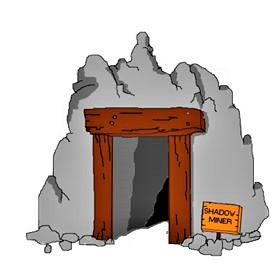
\includegraphics[%
			keepaspectratio]{../images/icone.jpg}%
			\vfill
		}
	}
}

\fboxrule=2pt
\newcommand\cincludegraphics[2][]{%
  \setbox0=\hbox{\includegraphics[#1]{#2}}%
  \abovebaseline[-.5\ht0]{\includegraphics[#1]{#2}}}

  
\renewcommand{\baselinestretch}{1}
\renewcommand{\partname}{}


\title{\textbf{{\Huge Manuel d'utilisation}}}
\author{
	\\
	\bsc{{\LARGE \bf ShadowMiner}} \\ \\ \\
	\bsc{{\LARGE \bf par ACCEr}} \\ \\
}
\date{{\LARGE \today}}

\pagestyle{fancy}
%\fancyfoot[L]{
\includegraphics{../images/ShadowMiners_logo_mini.png}} %50x33
\fancyfoot[L]{\cincludegraphics[scale=0.1]{../images/ShadowMiners_logo.png}} %50x33
\fancyfoot[R]{STRASBOURG 2022}
\fancyhead[R]{ACCEr}
\fancyhead[L]{Manuel d'utilisation}

\setcounter{tocdepth}{3}

\begin{document}
\AddToShipoutPicture*{\BackgroundPic}

\maketitle
\tableofcontents

%################### Garantie

\fancypagestyle{plain}{}
\stepcounter{chapter}
\part{Garantie} 

\section*{ASSISTANCE TECHNIQUE}
\paragraph*{} \hspace{0pt}
Si vous rencontrez des problèmes techniques, rendez-vous sur 
\url{https://accer.ddns.net/?p=support} pour obtenir les dernières informations de 
contact et des réponses aux questions les plus fréquentes. L'assistance est
disponible sur Internet. \\

\section*{GARANTIE LOGICIEL LIMITÉE ET ACCORD DE LICENCE}
\paragraph*{} \hspace{0pt}
Cette garantie logiciel limitée et cet accord de licence peuvent être mis à
jour régulièrement. La dernière version en date sera postée sur le site 
\url{https://accer.ddns.net/?p=report}. Vous devez toutefois retélécharger le 
jeu à chaque nouvelle version du jeu. Votre utilisation du Logiciel après la
publication d'un accord révisé constitue votre acceptation de ses termes. \\

LE "LOGICIEL" COMPORTE TOUS LES LOGICIELS INCLUS DANS LE PRÉSENT ACCORD, LE 
MANUEL D'UTILISATION, L'EMBALLAGE ET D'AUTRES SUPPORTS ÉCRITS, DOSSIERS,
SUPPORTS OU DOCUMENTATIONS ÉLECTRONIQUES OU EN LIGNE, ET TOUTES LES COPIES
DES DITS LOGICIELS ET DE LEURS SUPPORTS. \\

\section*{CONTENU CRÉÉ PAR L'UTILISATEUR}
\paragraph*{} \hspace{0pt}
Le logiciel peut autoriser l'utilisateur à créer du contenu : 
des cartes, des captures d'écran, un objet ou des vidéos des séquences de jeu. \\
En échange de l'utilisation du logiciel, et à condition que vos contributions
lors de l'utilisation du logiciel soient en accord avec les droits en vigueur, 
vous cédez par la présente au donateur de licence un droit internationnal
exclusif, perpétuel, irrévocable, entièrement transférable et sous-licenciable
d'utilisation, de quelque manière que ce soit, de vos contributions au logiciel
et à ses produits et services dérivés, incluant, mais sans s'y limiter, les
droits de reproduction, copie, adaptation, modification, exécution, diffusion,
transmission ou communication au grand public de toutes les manières, qu'elles
soient connues ou inconnues, et de distribuer vos contributions sans aucun avis
préalable ni aucune compensation, quelle qu'elle soit, pour toute la durée de la protection acordée
par les droits sur la propriété intellectuelle, en application des lois et des
conventions internationales. \\


\section*{CONNEXION À INTERNET}
\paragraph*{} \hspace{0pt}
Le logiciel peut nécessiter une connexion à Internet pour accéder aux
caractéristiques en ligne, à son authentification ou à d'autres fonctionnalités. \\
 

\section*{COMPTES UTILISATEURS}
\paragraph*{} \hspace{0pt}

Afin d'utiliser le logiciel ou une fonctionnalité de celui-ci, ou pour que
certaines fonctionnalités du logiciel fonctionnent correctement, il peut être
nécessaire de disposer d'un compte utilisateur sur un service en ligne.
Le logiciel peut aussi nécessiter la création d'un compte utilisateur
afin d'y avoir accès dans son intégralité. Vous êtes responsable de
l'usage et de la sécurité de vos comptes utilisateurs dont vous vous servez
pour accéder au logiciel et pour l'utiliser. \\


\section*{COLLECTE ET UTILISATION DES INFORMATIONS}
\paragraph*{} \hspace{0pt}
Par l'installation et l'utilisation du logiciel, vous acceptez les conditions
de collecte et d'utilisation des informations établies dans cette section, y
compris le transfert de toutes informations personnelles et autres à toutes
institutions, qu'elles quelles soient; l'affichage public de vos données, comme
l'identification du contenu que vous avez créé ou l'affichage de vos scores,
classements ou autres données du jeu avec les fabricants de matériel. \\

%################### Garantie

\newpage

%################### Installationn

\fancypagestyle{plain}{}
\stepcounter{chapter}
\part{Installation} 

\section{Depuis le CD-ROM}
\paragraph*{} \hspace{0pt}
Insérer le CD-ROM dans votre lecteur de disque. \\
Si l'installateur ne se lance pas, lancer l'éxécutable présent sur le disque. \\
Sélectionner ensuite la langue d'installation. \\
Vous pouvez ensuite choisir le dossier d'installation du jeu 
(par défault : C:\textbackslash Program Files (x86)\textbackslash ShadowMiner\textbackslash). \\
L'installateur vous proposera de changer le nom du racourci. \\
Vous pourrez ensuite choisir si vous souhaitez créer un racourci sur le bureau. \\
Un récapitulatif de l'installation vous sera présenté et vous pourrez ensuite cliquer sur "installer". \\
A la fin de l'installation, vous pourrez lancer le jeu directement. \\

\section{Depuis le site internet}
\paragraph*{} \hspace{0pt}
Télécharger l'installateur du jeu depuis la page \url{https;//accer.dddns.net/?p=download}. \\
Lancer l'installateur et suivez les mêmes étapes que pour l'installation depuis le CD-ROM. \\


%################### Installation

\newpage

%################### Désinstallation

\fancypagestyle{plain}{}
\stepcounter{chapter}
\part{Déinstallation} 

Pour désinstaller le jeu, il suffit d'exécuter le fichier unins000.exe. 
Il se situe dans le dossier d'installation du jeu. Pour y accéder, faîtes un clic droit sur le 
raccourci du jeu puis « propriétés » puis « emplacement du fichier » (par défaut vous trouverez le jeu dans 
C:\textbackslash Program Files (x86)\textbackslash ShadowMiner\textbackslash). 
Une popup vous demandera une confirmation.\\

%################### Déinstallation

\newpage

%################### Commande

\fancypagestyle{plain}{}
\stepcounter{chapter}
\part{Commande} 
\paragraph*{} \hspace{0pt}
Les commandes peuvent être modifiées dans les paramètres. \\ La configuration par défaut est : \\
{\begin{itemize}
	\item attaquer : Clic gauche de la souris
	\item avancer : Z
	\item reculer : S
	\item aller à droite : D
	\item aller à gauche : Q
	\item sauter : espace
	\item courir : maj (ou shift)
	\item interagir :  E \\
\end{itemize}}

%################### Commande

\newpage

%################### Démarrage

\fancypagestyle{plain}{}
\stepcounter{chapter}
\part{Démarrage}
\paragraph*{} \hspace{0pt}
Pour commencer à jouer, double cliquez sur l’icône du jeu sur votre bureau (si vous avez décoché le raccourci sur 
le bureau lors de l'installation, vous pouvez lancer le jeu depuis le menu de démarrage de WINDOWS en recherchant ShadowMiner). 
Une fois le jeu lancé un menu s'affichera. Si vous possédez une connexion à Internet et que vous souhaitez pouvoir 
partager votre progression via le site officiel du jeu, nous vous conseillons de vous connecter en cliquant sur le 
bouton « My Account » puis de vous inscrire ou de vous connecter à votre profil déjà existant. \\


\paragraph*{} \hspace{0pt}
Une fois de retour dans le menu, ou si vous ne vous êtes pas connecté, vous pouvez modifier vos paramètres 
de jeu (contrôles, résolution, son...) dans le menu « Settings ». \\


\paragraph*{} \hspace{0pt}
Maintenant que vous êtes fin prêt, vous pouvez lancer l'aventure en mode solo, ou si vous êtes connecté rejoindre 
ou lancer une partie multijoueur. \\ Bon jeu ! \\


%################### Démarrage

\newpage

%################### Menu

\fancypagestyle{plain}{}
\stepcounter{chapter}
\part{Menu} 
\paragraph*{} \hspace{0pt}
Dans le menu il y a 10 boutons : \\
{\begin{itemize}
	\item « Solo » : Ouvre l'écran de séléction des niveaux (voir « jeu hors-ligne » ci-dessous)
	\item « Multiplayer » : Ouvre l'écran de lobby avec les différentes parties déjà en cours et 
		un bouton pour en créer une soi-même (voir « jeu en ligne » ci-dessous)
	\item « Custom Map » : Permet de tester les niveaux créés par les autres joueurs si vous êtes connecté.
	\item « Map Editor » : Permet de créer votre propre niveau et de le partager avec les autres joueurs ! 
		Vous pourrez le sauvegarder sur votre ordinateur (et sur le serveur si vous êtes connecté).
	\item « My Account » :  Permet d'accéder à votre profil et de le personnaliser avec un pseudo et une description. 
		Vous pouvez également changer vos informations de base (prénom, nom, description et mot de passe).
	\item « My Progress » : Affiche la progression du joueur, c'est-à-dire le nombre de niveaux terminés 
		en solo, le nombre de parties gagnées en multijoueur et la date et l'heure de la dernière mise à jour 
		de ces statistiques.
	\item « Open website » : Ouvre le site du jeu directement dans votre navigateur par défaut (voir la partie 
		« le site web » ci-dessous).
	\item « Settings » : Permet de configurer les contrôles et de modifier le volume sonore, la résolution, la fréquence 
		et la qualité du jeu. On peut aussi basculer en plein écran ou non. Le dernier onglet permet de réinitialiser 
		TOTALEMENT le jeu, vous perdrez donc tout ce qui n'est pas enregistré sur le serveur (progression des niveaux, 
		terrains personnels, touches modifiées, etc...).
	\item « Credits » : Fait défiler les membres du groupe ACCEr et autres entités que nous remercions pour avoir 
		rendu possible l'élaboration de ce projet possible.
	\item « Exit » :  Ferme le jeu, tout simplement !  \\
\end{itemize}}

%################### Menu

\newpage

%################### mode jeu

\fancypagestyle{plain}{}
\stepcounter{chapter}
\part{Les modes de jeu} 

\section{Jeu hors ligne}
\paragraph*{} \hspace{0pt}
Le mode solo est constitué de 20 niveaux avec une difficulté croissante. 
Chaque niveau (niveau 1 exclu) se débloque lorsque le précédent est terminé. 
Ce mode ne nécessite pas de connexion internet et la progression est sauvegardée sur l'ordinateur de l'utilisateur. \\

\section{Jeu en ligne} 
\paragraph*{} \hspace{0pt}
Ce mode se joue à trois joueurs. Deux personnes incarnent les mineurs qui doivent échapper au ShadowMiner, 
contrôlé par le troisième joueur. Les mineurs doivent survivre pendant 2 minutes et 30 secondes 
sans se faire tuer, sinon le ShadowMiner gagne. \\

%################### mode jeu

\newpage

%################### Les personnages

\fancypagestyle{plain}{}
\stepcounter{chapter}
\part{Les personnages} 

\section{Le mineur}
\paragraph*{} \hspace{0pt}
Le personnage que vous incarnez est un mineur. Il s'appelle Dananau et vit en Moldavie dans la ville 
de Giurgiulești. Il vit avec sa femme Marinela et sa fille Anastacia. 
Depuis trois ans, il travaille dans la mine située près de la ville. \\

\section{Le ShadowMiner}
\paragraph*{} \hspace{0pt}
Personne ne sait d'où il vient, ni ses intentions. C'est un monstre vert, errant dans la mine qui attaque tout ce qui est vivant. 
Malheureusement pour vous, il n'y a personne d'autre pour le distraire. \\

%################### Les personages

\newpage

%################### Site

\fancypagestyle{plain}{}
\stepcounter{chapter}
\part{Site internet} 
\paragraph*{} \hspace{0pt}
L'adresse du site est \url{https://accer.ddns.net}. Comme le jeu est réalisé dan un cadre scolaire, 
vous pouvez y trouver les différents rapports de soutenance, ainsi que le cahier des charges, la 
répartition des tâches, les sources utilisées et le planning d'avancement. Il y a aussi le trailer 
du jeu, le classement des meilleurs joueurs, un outil de discussion en direct pour les joueurs,  
une partie consacrée à l'assistance et bien sûr, une page de téléchargement du jeu. \\

%################### Site

\newpage

%################### Crédits

\fancypagestyle{plain}{}
\stepcounter{chapter}
\part{Crédits} 
\paragraph*{Programation : } \hspace{0pt}
ACCEr :
Antoine CLAUDEL, 
Cédric FARINAZZO, 
Clément LANGUERRE et  
Edgar GRIZZI \\

\paragraph*{Chef de projet : } \hspace{0pt}
Cédric FARINAZZO \\

\paragraph*{Concept : } \hspace{0pt}
Clément LANGUERRE \\

\paragraph*{Son : } \hspace{0pt}
Cédric FARINAZZO, 
Edgar GRIZZI et 
Nicolas MASCIOCCHI \\

\paragraph*{Graphismes : } \hspace{0pt}
Antoine CLAUDEL, 
Clément LANGUERRE et 
Edgar GRIZZI \\

\paragraph*{Conception des maps : } \hspace{0pt}
Antoine CLAUDEL, 
Clément LANGUERRE, 
Cédric FARINAZZO \\

\paragraph*{Conception des préfabs : } \hspace{0pt}
Antoine CLAUDEL, 
Clément LANGUERRE et 
Cédric FARINAZZO \\

\paragraph*{Multijoueur : } \hspace{0pt}
Cédric FARINAZZO \\

\paragraph*{IA : } \hspace{0pt}
Cédric FARINAZZO \\

\paragraph*{Site internet : } \hspace{0pt}
Cédric FARINAZZO \\

\paragraph*{Cinématique : } \hspace{0pt}
Cédric FARINAZZO et 
Clément LANGUERRE \\

\paragraph*{Trailer : } \hspace{0pt}
Clément LANGUERRE \\

\paragraph*{Remerciements à : } \hspace{0pt}
Pierre KELBERT, 
Sébastien HOEHN et 
Anass KASMI \\

\paragraph*{Aide : } \hspace{0pt}
EPITA, 
Google, 
Pixabay, 
Asset store, 
OpenClassroom, 
UPLN, 
TutoUnityFR, 
Unity-Technologies et 
Git \\

\paragraph*{Test : } \hspace{0pt}
Antoine CLAUDEL, 
Cédric FARINAZZO, 
Clément LANGUERRE, 
Edgar GRIZZI et 
Anass KASMI \\


%################### Crédits

%################### Secrets

\fancypagestyle{plain}{}
\stepcounter{chapter}
\part{Secrets} 
\paragraph*{} \hspace{0pt}
Le Konami Code est présent dans le menu du jeu. \\ \\
Si vous trouvez le chargement un peu long, la touche Echap permet de l'accélérer. \\


%################### Secrets

\end{document}